\chapter{Psalm 75}

\begin{figure}
  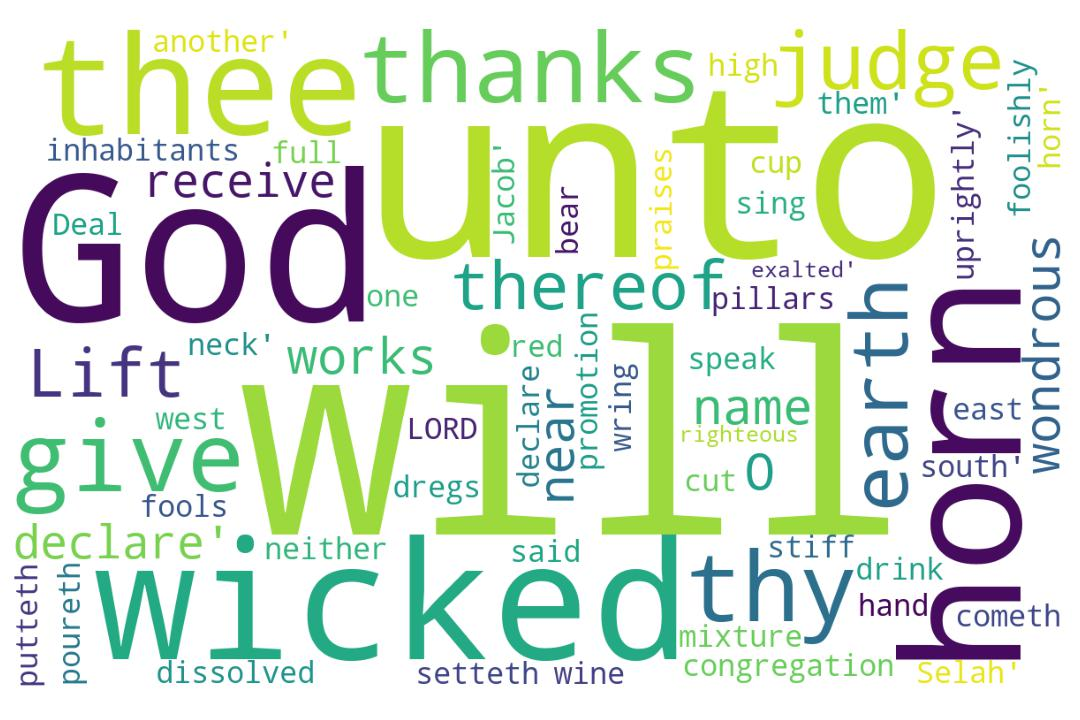
\includegraphics[width=\linewidth]{19OT-Psalms/Psalm75-WordCloud.jpg}
  \caption{Psalm 75 Word Cloud}
  \label{fig:Psalm 75 word Cloud}
\end{figure}

\marginpar{\scriptsize \centering \fcolorbox{bone}{lime}{\textbf{A WORTHY GOD}}\\ (Psalm 75:1-10) \begin{compactenum}[I.][8]
    \item A \textbf{Worthy Declaration} \index[scripture]{Psalms!Psa 075:01}(Psa 75:1)
    \item \textbf{Works on Display} \index[scripture]{Psalms!Psa 075:01}(Psa 75:1)
    \item (Sinful) \textbf{World Dissolved} \index[scripture]{Psalms!Psa 075:03}(Psa 75:3)
    \item \textbf{Weighty Decisions} \index[scripture]{Psalms!Psa 075:07}(Psa 75:7)
     \item A \textbf{Wrathful Drink} (The Cup) \index[scripture]{Psalms!Psa 075:08}(Psa 75:8)
     \item The \textbf{Wringing out of Dregs} \index[scripture]{Psalms!Psa 075:08}(Psa 75:8)
   \item (The) \textbf{Wicked Destroyed} \index[scripture]{Psalms!Psa 075:10}(Psa 75:10)
\end{compactenum}}
    
\marginpar{\scriptsize \centering \fcolorbox{bone}{yellow}{\textbf{THE JUDGMENT}}\\ (Psalm 75:1-10) \begin{compactenum}[I.][8]
    \item The \textbf{Declaration} \index[scripture]{Psalms!Psa 075:01} \index[scripture]{Psalms!Psa 075:09}(Psa 75:1, 9)
    \item \textbf{Dealings} \index[scripture]{Psalms!Psa 075:04} (Psa 75:4)
    \item \textbf{Dissolution} \index[scripture]{Psalms!Psa 075:05} (Psa 75:5)
    \item \textbf{Directions} \index[scripture]{Psalms!Psa 075:06} (Psa 75:6) (Look North!)
    \item \textbf{Dregs} \index[scripture]{Psalms!Psa 075:08} (Psa 75:8) 
    \item The \textbf{Drinking} \index[scripture]{Psalms!Psa 075:08} (Psa 75:8) 
    \item The \textbf{Defeat} \index[scripture]{Psalms!Psa 075:10} (Psa 75:10) 
\end{compactenum}}
    




% \textcolor[cmyk]{0.99998,1,0,0}{
\footnote{\textcolor[rgb]{0.00,0.25,0.00}{\hyperlink{TOC}{Return to end of Table of Contents.}}}\footnote{\href{https://audiobible.com/bible/psalms_75.html}{\textcolor[cmyk]{0.99998,1,0,0}{Psalm 75 Audio}}}\textcolor[cmyk]{0.99998,1,0,0}{To the chief Musician, Al-taschith, A Psalm \emph{or} Song of Asaph.}\\
\\
\textcolor[cmyk]{0.99998,1,0,0}{Unto thee, O God, do we give thanks, \emph{unto} \emph{thee} do we give thanks: for \emph{that} thy name is near thy wondrous \fcolorbox{bone}{lime}{works} declare.}
[2] \textcolor[cmyk]{0.99998,1,0,0}{When I shall receive the congregation I will judge uprightly.}
[3] \textcolor[cmyk]{0.99998,1,0,0}{The earth and all the inhabitants thereof are \fcolorbox{bone}{lime}{dissolved}: I bear up the pillars of it. Selah.}\footnote{\textbf{1 Peter 3:11-12} - Seeing then that all these things shall be dissolved, what manner of persons ought ye to be in all holy conversation and godliness, [12] Looking for and hasting unto the coming of the day of God, wherein the heavens being on fire shall be dissolved, and the elements shall melt with fervent heat?}
[4] \textcolor[cmyk]{0.99998,1,0,0}{I said unto the fools, Deal not foolishly: and to the wicked, Lift not up the horn:}
[5] \textcolor[cmyk]{0.99998,1,0,0}{Lift not up your horn on high: speak \emph{not} \emph{with} a stiff neck.}
[6] \textcolor[cmyk]{0.99998,1,0,0}{For promotion \emph{cometh} neither from the east, nor from the west, nor from the south.}
[7] \textcolor[cmyk]{0.99998,1,0,0}{But God \emph{is} \fcolorbox{bone}{lime}{the judge}: he putteth down one, and setteth up another.}
[8] \textcolor[cmyk]{0.99998,1,0,0}{For in the hand of the LORD \emph{there} \emph{is} a cup, and the wine is red; it is \fcolorbox{bone}{lime}{full of mixture}; and he poureth out of the same: but the dregs thereof, all the wicked of the earth shall \fcolorbox{bone}{lime}{wring} \emph{them} out, \emph{and} drink \emph{them}.}
[9] \textcolor[cmyk]{0.99998,1,0,0}{But I will declare for ever; I will sing praises to the God of Jacob.}
[10] \textcolor[cmyk]{0.99998,1,0,0}{All the horns of the \fcolorbox{bone}{lime}{wicked} also will I cut off; \emph{but} the horns of the righteous shall be exalted.}\footnote{See the horns of \textbf{Revelation 13:1} - And I stood upon the sand of the sea, and saw a beast rise up out of the sea, having seven heads and ten horns, and upon his horns ten crowns, and upon his heads the name of blasphemy. ``Horns'' indicate powers.} 